\section{Methods}

The algorithm we developed can be utilised to identify regions of parameter space capable of producing a desired stability while handling uncertainty in biochemical rate constants and initial conditions. It can be used to design new systems of desired stability or study the stability of existing systems. The method we are presenting here is based on the Approximate Bayesian Computation, Sequential Monte Carlo method (ABC SMC), a statistical inference method developed by \textcite{Toni:2009tr}. This simulation-based method, using an iterative process can arrive at a distribution of parameter values that can give rise to a desired system behaviour. 

ABC methods are used for inferring the posterior distribution in cases where it is too computationally hard to evaluate the likelihood function. Instead of calculating the likelihood, ABC methods simulate the data and then compare the desired to the simulated data \autocite{Toni:2009tr}. Given the prior distribution $\pi(\theta)$ we can approximate the posterior distribution, $\pi(\theta\mid x)\propto f(x\mid\theta)\pi(\theta)$, where $f(x\mid\theta)$ is the likelihood of a parameter, $\theta$, given the data, $x$. There are a number of different variations of the ABC algorithm. The generic ABC algorithm is as follows:
	
	\begin{algorithm}[h]
	\label{alg:ABC}
  \caption{Generic ABC algorithm}
 \begin{algorithmic}[1]
    \Statex
	\State Sample a parameter vector $\theta$ from prior $\pi(\theta)$
	\State Simulate the model given $\theta$
    \State Compare the simulated data with the desired data, using a distance function $d$ and tolerance $\epsilon$. if $d \leq \epsilon$, accept $\theta$ 
   
  \end{algorithmic}
\end{algorithm}


The simplest ABC algorithm is the ABC rejection sampler \autocite{Pritchard:1999td}. In this method, parameters are sampled and simulated, and for each sample if the distance from that to the desired behaviour is greater than a threshold, the sample is rejected, otherwise accepted. The main disadvantage of this method is that if the prior distribution is very different from the posterior, the acceptance rate is very low \autocite{Toni:2009tr}. %An alternative method is the ABC Markov Chain Monte Carlo (MCMC) developed by \textcite{Marjoram:2003up}. The disadvantage of this method is that if it gets stuck in an area of low probability it can be very slow to converge.

The method used here, developed by \textcite{Toni:2009tr} is the ABC SMC method that avoids both these issues faced by the above methods. It propagates the prior through a series of intermediate distributions in order to arrive to an approximation of the posterior. The tolerance, $\epsilon$ for the distance of the simulated data to the desired data is made smaller at each iteration. When $\epsilon$ is sufficiently small, the result will approximate the posterior distribution \autocite{Toni:2009tr}. 

In the algorithm we developed the desired behaviour in ABC SMC is replaced by a desired stability that the simulated model has to have to be accepted. The $\epsilon$ measures the distance of the current stability to the desired stability. The advantages of this method is that it can handle stochastic as well as deterministic models, and can inherently handle parameter uncertainty \autocite{Barnes:2011hh}. The algorithm is summarised in Algorithm~ \ref{alg:StabilityFinder} below.

\begin{algorithm}[htbp]
\label{alg:StabilityFinder}
\caption{StabilityFinder algorithm}
 \begin{algorithmic}[1]
    \Statex
	\State Initialise $\epsilon$ 
	\Let{population p}{1}
	\If{p $= 1$}
		\State Sample particles ($\theta$) from priors
		\Else
			\State Sample particles from previous population
			\State Perturb each particle by $\pm$ half the range of the previous population (j) to obtain new perturbed population (i).
	\EndIf
	\State Sample initial conditions via Latin Hypercube Sampling.
    \State Simulate each particle to obtain steady state values.
    \State Cluster steady state
	\State Reject particles if d $\textgreater$ $\epsilon$.
    \State Calculate weight for each accepted $\theta$
	\State $w_{t}^{(i)} = \begin{cases} 1, & \mbox{if } p = 0 \\\frac{\pi(\theta_{t}^{(i)})}{\sum_{j=1}^N w_{t-1}^{(j)} K_{t}(\theta_{t-1}^{(j)}, \theta_{t}^{(i)})}, & \mbox{if } p \geq  0. \end{cases}$
	\State Normalise weights
	\Repeat {steps 3 - 15} \Until{$\epsilon \leq \epsilon_T$}
  \end{algorithmic}
\end{algorithm}



%Given a prior distribution of values for each parameter in the model $\pi(\theta)$, and a desired behaviour, which in our case is model stability, can arrive at the posterior distributions $\pi(\theta|d(s_0, s*)\leq \epsilon_T)$. The tolerance $\epsilon$ represents the distance between the target behaviour and the current simulated behaviour. As this $\epsilon$ gradually becomes smaller, the distributions get nearer to the target distribution capable of giving rise to the desired behaviour \autocite{Toni:2009tr}. The advantages of this method is that it can handle stochastic as well as deterministic models, and can inherently handle parameter uncertainty \autocite{Barnes:2011hh}. The algorithm can be summarised as seen in Figure~\ref{fig:flowchart}.

We packaged this algorithm into a python package, called StabilityFinder.  The user provides the model file, in the form of SBML of cuda as well as the input file. The user input file contains all the necessary information to run the algorithm that is not contained in the model itself. The user specifies the desired stability, the total variance as well as the variance within each cluster that . In addition the user provides the tolerance for the distance from the desired behaviour necessary for the algorithm to terminate. The flow of execution is illustrated in Figure~\ref{fig:flowchart} below.

\clearpage
\begin{figure}[htbp]
	\centering
	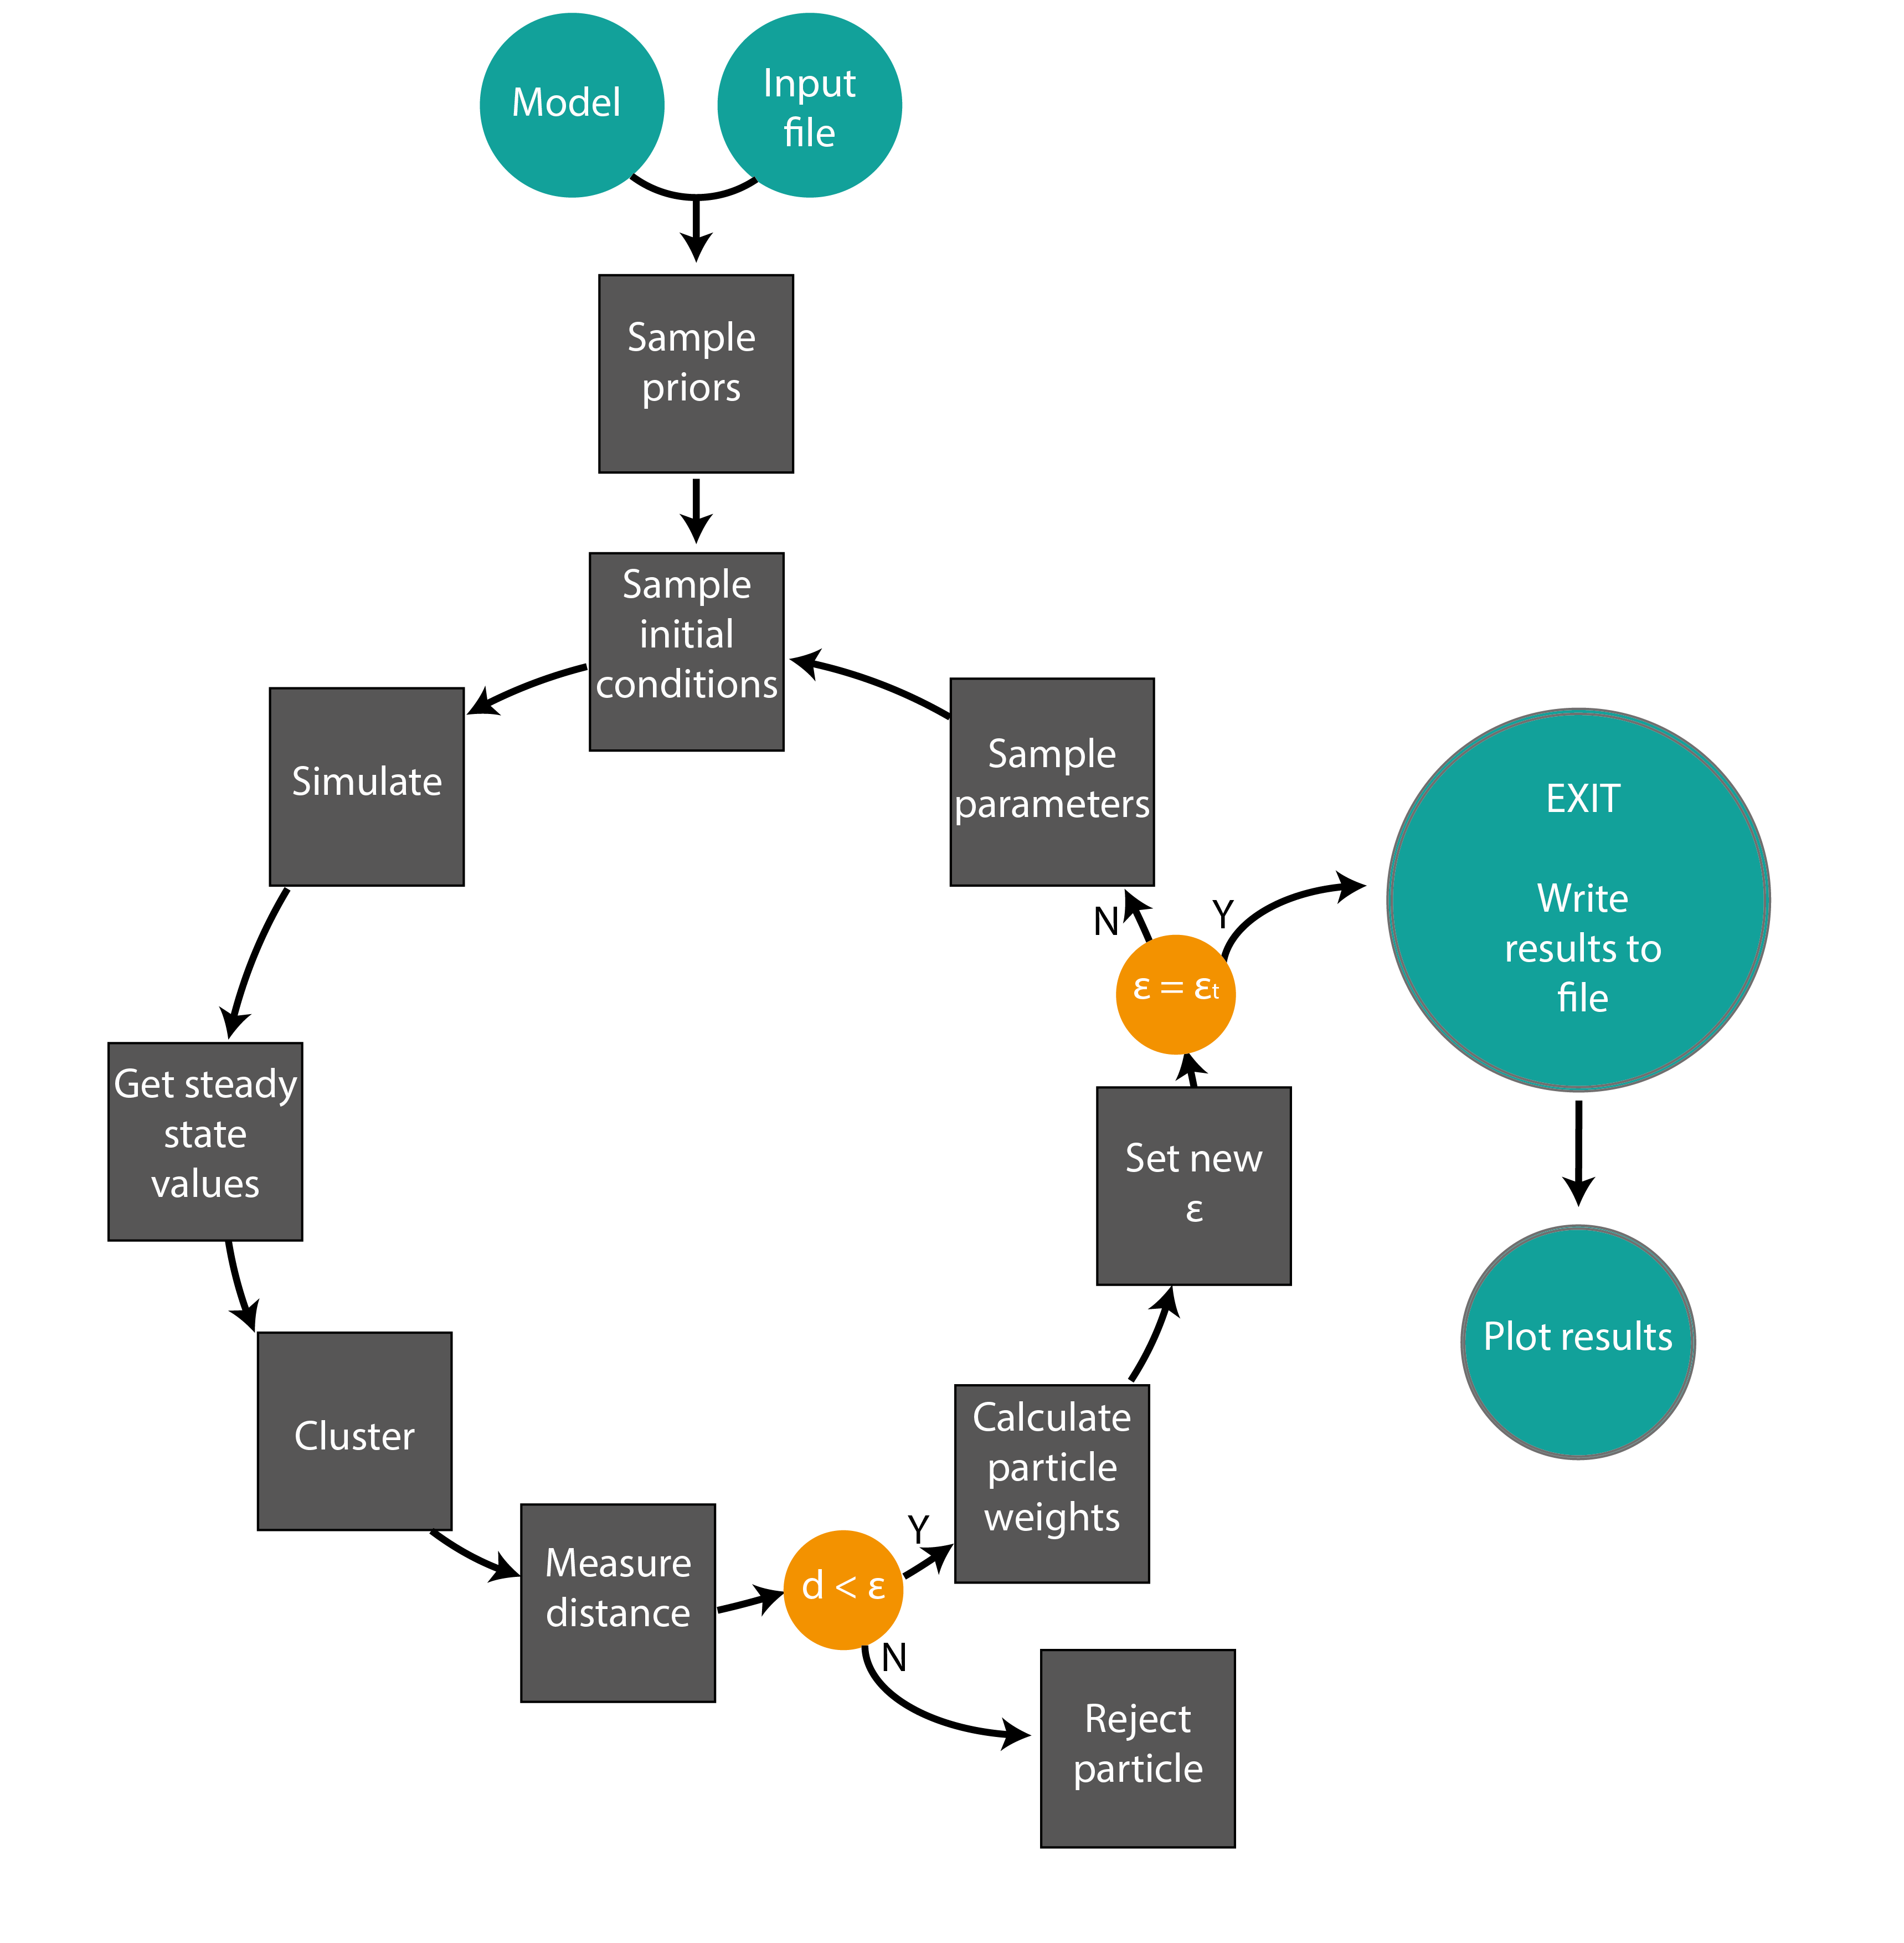
\includegraphics[scale=0.6]{chapterModelling/images/StabilityChecker_flowchart-01}
	\caption[Flowchart of the algorithm used in StabilityFinder]{Flowchart of the algorithm used in StabilityFinder. $\epsilon$ stands for the threshold for the distance from the desired value.}
	\label{fig:flowchart}
\end{figure}
\clearpage
 
StabilityFinder begins by sampling from the prior, by selecting a random value from within the user-specified range. Each sample from the priors is called a particle. The number of particles is specified in the user input file. The algorithm then proceeds by sampling initial conditions using Latin Hypercube sampling that ensures an even coverage of values from within the specified range. The model is then simulated for each parameter sample set, for each initial condition set.  It uses cuda-sim software \autocite{Zhou:2011hp} to simulate the models thus taking full advantage of GPUs.  As soon as the simulations are complete, the steady state values for the two species of interest are clustered in order to determine the stability achieved by each parameter sample set. Whether the model has been simulated using ODEs or the Gillespie algorithm dictates the method of clustering used. The two algorithms are summarised in the Appendix. Once the number of clusters present for each parameter set has been determined, the distance from the desired values is measured. If the distance between the simulation and the target behaviour is greater than a predefined threshold distance $\epsilon$, then the parameter values that produced that simulation are rejected. The tolerated distance is first calculated from the samples taken, and then decreased at each iteration until it reaches the final accepted tolerance. This is repeated for a predefined number of samples which are collectively referred to as a population. Each particle in a population has a weight associated with it, which represents the probability of it producing the desired behaviour. At subsequent iterations the new samples are obtained from the previous populations and the $\epsilon$ is set to smaller value, thus eventually reaching the desired behaviour. 
 
\subsection{Calculating robustness}

We use the results from StabilityFinder to estimate system robustness, by comparing the volume of the posterior to the volume of the prior in a given model. Here we are calculating it using a Monte Carlo sampling accept reject algorithm. Taking a number of random samples from the prior, it keeps track of how many are also found in the functional region $F$ of the posterior. The ones that are found in $F$ are accepted and the rest rejected. Robustness is then defined as the number of accepted samples divided by the total number of samples.
\begin{algorithm}[ht]
	\label{alg:robustness}
  \caption{Calculating robustness via Monte Carlo sampling rejection }
 \begin{algorithmic}[1]
    \Statex
    \State Sample from priors 
    \State Get min and max boundaries of functional region of posterior ($F$)
	\If{sample within $F$}
    	\State $accepted += 1$
    \EndIf
    	    	
    \State $acceptance\_rate$ = $\frac{accep
    	ted}{number of samples}$
    \State \Return $acceptance\_rate$
    
  \end{algorithmic}

\end{algorithm}

\newpage






